% !TEX program = xelatex
\documentclass[10pt,letterpaper,twocolumn]{article}

% === GEOMETRY ===
% Bottom margin + footskip tuned so the page number sits ≥0.6in from the
% sheet edge — clear of consumer-inkjet unprintable zones (HP DeskJet
% bottom dead strip is 0.5in) without scaling the page down.
\usepackage[top=0.75in, bottom=0.75in, left=0.75in, right=0.75in, footskip=12pt]{geometry}

% === FONTS ===
\usepackage{fontspec}
\usepackage{unicode-math}
\setmainfont{Latin Modern Roman}[
  Extension=.otf,
  UprightFont=lmroman10-regular,
  BoldFont=lmroman10-bold,
  ItalicFont=lmroman10-italic,
  BoldItalicFont=lmroman10-bolditalic,
]
\setsansfont{Latin Modern Sans}[
  Extension=.otf,
  UprightFont=lmsans10-regular,
  BoldFont=lmsans10-bold,
  ItalicFont=lmsans10-oblique,
  BoldItalicFont=lmsans10-boldoblique,
]
\setmonofont{Latin Modern Mono}[
  Extension=.otf,
  UprightFont=lmmono10-regular,
  ItalicFont=lmmono10-italic,
  Scale=0.85,
]
% YWFT Processing is used in exactly ONE place: the title in the header.
% Its punctuation glyphs are unreliable (the "/" renders as an ampersand-
% like mark), so body text, subtitle, and the edition slot stay in the
% Latin Modern faces.
\newfontfamily\acbold{ywft-processing-bold}[
  Path=../../system/public/type/webfonts/,
  Extension=.ttf
]

% === PACKAGES ===
\usepackage{xcolor}
\usepackage{colortbl}
\usepackage{titlesec}
\usepackage{enumitem}
\usepackage{booktabs}
\usepackage{tabularx}
\usepackage{fancyhdr}
\usepackage{hyperref}
\usepackage{xurl}
\usepackage{graphicx}
\graphicspath{{./}{figures/}}
\usepackage{ragged2e}
\usepackage{microtype}
\usepackage[font=footnotesize]{caption}
\usepackage{natbib}
\usepackage{tikz}
\usetikzlibrary{calc,positioning,shapes.geometric,arrows.meta}

% --- TikZ helpers for inline keyboard / hex / mapping diagrams ---
\definecolor{keyfill}{RGB}{248,248,250}
\definecolor{keystroke}{RGB}{160,156,170}
\definecolor{keymapped}{RGB}{180,72,135}
\definecolor{keysharp}{RGB}{52,52,64}
\tikzset{
  kcap/.style={draw=keystroke, fill=keyfill, rounded corners=0.6pt,
               minimum width=0.34cm, minimum height=0.34cm,
               inner sep=0pt, font=\scriptsize\sffamily},
  kcap mapped/.style={kcap, fill=keymapped!18, draw=keymapped!60,
                       text=keymapped!90},
  kcap sharp/.style={kcap, fill=keysharp, draw=keysharp,
                      text=white, font=\scriptsize\sffamily\bfseries},
  hexkey/.style={regular polygon, regular polygon sides=6,
                  draw=keystroke, fill=keyfill, rounded corners=0pt,
                  minimum size=0.55cm, inner sep=0pt,
                  font=\tiny\sffamily},
  hexkey mapped/.style={hexkey, fill=keymapped!22, draw=keymapped!70,
                          text=keymapped!90},
}
% === COLORS ===
\definecolor{acpink}{RGB}{180,72,135}
\definecolor{acpurple}{RGB}{120,80,180}
\definecolor{acdark}{RGB}{64,56,74}
\definecolor{acgray}{RGB}{119,119,119}
\definecolor{acblue}{RGB}{42,100,212}
\definecolor{acgreen}{RGB}{42,154,58}
\definecolor{acorange}{RGB}{216,120,0}
% Domain chip for the corollary table — small caps-ish bold colored tag
\newcommand{\dmn}[2]{\textcolor{#1}{\textbf{#2}}}
% Row QR code for the corollary table — links each object to its
% canonical home (Wikipedia, the project's own site, or its spec).
% PNGs generated by qrencode + magick PNG32 in figures/qr/.
% Centered on the row's text baseline so label text sits vertically
% centered against the tile.
\newcommand{\qrc}[1]{\raisebox{\dimexpr-0.5\height+0.8ex\relax}{\includegraphics[height=0.68cm]{figures/qr/#1.png}}}

% === HYPERREF ===
\hypersetup{
  colorlinks=true,
  linkcolor=acpurple,
  urlcolor=acpurple,
  citecolor=acpurple,
  pdfauthor={@jeffrey},
  pdftitle={Keymaps as Social Software: Versioned Virtual Objects via Social Contract},
}

% === SECTION FORMATTING ===
\titleformat{\section}
  {\normalfont\bfseries\normalsize\uppercase}
  {\thesection.}
  {0.5em}
  {}
\titlespacing{\section}{0pt}{1.2em}{0.3em}

\titleformat{\subsection}
  {\normalfont\bfseries\small}
  {\thesubsection}
  {0.5em}
  {}
\titlespacing{\subsection}{0pt}{0.8em}{0.2em}

% === HEADER/FOOTER ===
\pagestyle{fancy}
\fancyhf{}
\renewcommand{\headrulewidth}{0pt}
\fancyfoot[C]{\footnotesize\thepage}
% Full-page table spread: folio moves to the bottom right so it can't
% collide with the table body.
\fancypagestyle{tablefolio}{%
  \fancyhf{}%
  \renewcommand{\headrulewidth}{0pt}%
  \fancyfoot[R]{\footnotesize\thepage}%
}

% === LIST SETTINGS ===
\setlist[itemize]{nosep, leftmargin=1.2em, itemsep=0.1em}
\setlist[enumerate]{nosep, leftmargin=1.2em}

% === COLUMN SEPARATION ===
\setlength{\columnsep}{1.8em}

% === PARAGRAPH SETTINGS ===
\setlength{\parindent}{1em}
\setlength{\parskip}{0.3em}

% Hyphenation for narrow two-column layout
\tolerance=800
\emergencystretch=1em
\hyphenpenalty=50

\newcommand{\acdot}{{\color{acpink}.}}
% Every dot in Aesthetic.Computer is the AC pink dot, inline too.
\newcommand{\ac}{Aesthetic{\acdot}Computer}
% Keycap chip — the one canonical inline key glyph: cap-height box
% (no descender slack, so it sits low in the text line) with a gray
% bottom-shadow bezel, like the keycaps in the figures.
\DeclareRobustCommand{\key}[1]{\tikz[baseline=(k.base)]{%
  \node[fill=keystroke, rounded corners=1.3pt, inner xsep=2.4pt,
        inner ysep=1.9pt, anchor=base, yshift=-1.2pt] at (0,0)
    {\footnotesize\ttfamily\bfseries\vphantom{A}\phantom{#1}};
  \node[draw=keystroke, line width=0.4pt, fill=keyfill,
        rounded corners=1.3pt, inner xsep=2.4pt, inner ysep=1.9pt,
        anchor=base] (k) at (0,0)
    {\footnotesize\ttfamily\bfseries\vphantom{A}#1};}}
% A run of keycaps with even spacing: \keys{C,D,E,F,G,A,B}
\makeatletter
\DeclareRobustCommand{\keys}[1]{{\def\sep{}\@for\kk:=#1\do{\sep\key{\kk}\def\sep{\,}}}}
\makeatother

\begin{document}

\twocolumn[{%
\begin{center}
{\acbold\fontsize{27pt}{31pt}\selectfont\color{acdark} Keymaps as Social Software}\par
\vspace{0.5em}

\includegraphics[width=0.7\textwidth]{figures/cover}\par
\vspace{0.4em}
{\itshape\fontsize{14.5pt}{17pt}\selectfont\color{acpink} Versioned Virtual Objects via Social Contract}\par
\vspace{0.5em}
{\small\color{acgray} \href{https://prompt.ac/@jeffrey}{@jeffrey} \,$\cdot$\, Aesthetic{\acdot}Computer \,$\cdot$\, ORCID \href{https://orcid.org/0009-0007-4460-4913}{0009-0007-4460-4913}}\par
\vspace{0.6em}
{\color{acpink}\rule{\textwidth}{1.2pt}}
\vspace{0.5em}
\end{center}

\begin{quote}
\small\noindent\textbf{Abstract.}
A \emph{keymap} --- the small declarative table that says ``the QWERTY key \key{A} plays MIDI 60'' --- is software in every functional sense: versioned, invented, forked, and demanded across applications. But it is not a binary, not a project, not a service, and the open-source vs.\ proprietary axis cannot see it. I name the category \emph{social software} --- punning on Shirky, and joining the usage of McCarthy and Reas's UCLA initiative of that name, inside which this paper was written --- and trace it from Sholes to Colemak, Jankó to Wicki--Hayden, and into the unowned QWERTY-piano convention every major DAW ships. Read through Lialina's \emph{Turing Complete User}~\citep{lialina2012turing}, the keymap is the user-authorable gap whose closure is the disappearance of the user as author; I present the \texttt{notepat.com} keymap --- ``notes that name themselves'' --- as evidence that the gap is still open.
\end{quote}
\vspace{0.5em}
}]

\section{Introduction: An Artifact}

Figure~\ref{fig:notepat-keymap} is a one-page diagram of the keymap shipped by \texttt{notepat.com}, a chromatic keyboard instrument inside \ac{}. The diagram shows a piano keyboard up top, a QWERTY keyboard below, and dashed lines connecting the two. The connecting principle is the slogan the project ships under: \emph{notes that name themselves}. The QWERTY letter \key{C} plays C; \key{D} plays D; \key{E} plays E; and so on through \key{B}. The upper octave continues alphabetically (\keys{H,I,J,K,L,M,N} for $C_5$ through $B_5$). Sharps sit one row above their natural where possible, by analogy to piano black keys (\keys{V,S,W,R,Q} for $C^\sharp\,D^\sharp\,F^\sharp\,G^\sharp\,A^\sharp$).

\begin{figure*}[t]
\centering
% Native TikZ rendering of the notepat keymap diagram (Figure 1).
% Replaces the slide-pipeline PNG so the figure matches the paper's
% other vector diagrams. Piano keyboard (with the QWERTY letter that
% plays each note) above, QWERTY keyboard below, dashed color-matched
% connectors between the naturals. No hand labels — the hand split is
% carried by the two background tints and the caption.
% Key mapping verified against fedac/native/pieces/notepat.mjs and the
% AC Native screenshot: H I J K L M N = C5..B5 alphabetically (M=A5,
% N=B5), sharps V S W R Q (lower) and T Y U O P (upper).
\begingroup
% --- notepat note colors (from slides/notepat-keymap/template.html) ---
\definecolor{ncc}{HTML}{FF3232}\definecolor{ncd}{HTML}{FFA000}%
\definecolor{nce}{HTML}{FFE600}\definecolor{ncf}{HTML}{32C832}%
\definecolor{ncg}{HTML}{3278FF}\definecolor{nca}{HTML}{8232C8}%
\definecolor{ncb}{HTML}{B450FF}%
\definecolor{nCC}{HTML}{FF2850}\definecolor{nDD}{HTML}{FFB400}%
\definecolor{nEE}{HTML}{FFFF32}\definecolor{nFF}{HTML}{32FF64}%
\definecolor{nGG}{HTML}{32C8FF}\definecolor{nAA}{HTML}{B432FF}%
\definecolor{nBB}{HTML}{FF50FF}%
\definecolor{extbg}{HTML}{FFF4D6}\definecolor{extfg}{HTML}{8A7330}%
\definecolor{extbd}{HTML}{D4C075}%
\definecolor{extbk}{HTML}{5A4818}\definecolor{extbkfg}{HTML}{F8E7A0}%
\definecolor{octbg}{HTML}{F4ECFF}\definecolor{octfg}{HTML}{6B3FC0}%
\definecolor{octbd}{HTML}{B89DF0}%
\resizebox{\textwidth}{!}{%
\begin{tikzpicture}
% --- geometry ---
% piano: 17 white keys, pitch 1.02, key 0.98 x [4.4 .. 7.5]
% qwerty: caps 0.95, pitch 1.0, rows at y = 2.30 / 1.15 / 0
\def\pw{1.02}
\def\qx{2.45}
% --- piano key macros ---
\def\pkey#1#2#3#4{\begin{scope}[shift={({#1*\pw},0)}]
  \draw[acdark, fill=white, line width=0.8pt, rounded corners=1.5pt]
    (0,4.4) rectangle (0.98,7.5);
  \fill[#4] (0.04,4.44) rectangle (0.94,4.86);
  \draw[acdark!45, line width=0.4pt] (0.04,4.86) -- (0.94,4.86);
  % letter + note name live in the band BELOW the black keys
  \node[font=\large\ttfamily\bfseries, text=acdark] at (0.49,5.34) {#2};
  \node[font=\scriptsize\ttfamily, text=acdark!80] at (0.49,5.02) {#3};
\end{scope}}
\def\pkeyext#1#2#3{\begin{scope}[shift={({#1*\pw},0)}]
  \draw[extbd, dashed, fill=extbg, fill opacity=0.55, line width=0.8pt, rounded corners=1.5pt]
    (0,4.4) rectangle (0.98,7.5);
  \node[font=\large\ttfamily\bfseries, text=extfg, opacity=0.75] at (0.49,5.34) {#2};
  \node[font=\scriptsize\ttfamily, text=extfg, opacity=0.75] at (0.49,5.02) {#3};
\end{scope}}
\def\pbkey#1#2#3{\begin{scope}[shift={({#1},0)}]
  \draw[black, fill=black!92, line width=0.8pt, rounded corners=1.2pt]
    (-0.31,5.55) rectangle (0.31,7.5);
  \node[font=\normalsize\ttfamily\bfseries, text=white] at (0,6.98) {#2};
  \node[font=\fontsize{5.5pt}{5.5pt}\selectfont\ttfamily, text=white!75!black]
    at (0,6.45) {#3};
\end{scope}}
\def\pbkeyext#1#2#3{\begin{scope}[shift={({#1},0)}]
  \draw[extbk!80!black, dashed, fill=extbk, fill opacity=0.55, line width=0.8pt, rounded corners=1.2pt]
    (-0.31,5.55) rectangle (0.31,7.5);
  \node[font=\normalsize\ttfamily\bfseries, text=extbkfg, opacity=0.8] at (0,6.98) {#2};
  \node[font=\fontsize{5.5pt}{5.5pt}\selectfont\ttfamily, text=extbkfg!80]
    at (0,6.45) {#3};
\end{scope}}
% --- qwerty cap macros ---
% mapped natural: colored fill; #5 = label color (white or dark)
\def\qcap#1#2#3#4#5#6{\begin{scope}[shift={({#1},{#2})}]
  \draw[#4, fill=#3, line width=1pt, rounded corners=2.2pt]
    (0,0) rectangle (0.95,0.95);
  \node[font=\large\ttfamily\bfseries, text=#5] at (0.475,0.475) {\strut#6};
\end{scope}}
% sharp: near-black cap, border in the sharp's note color
\def\qsharp#1#2#3#4{\begin{scope}[shift={({#1},{#2})}]
  \draw[#3, fill=black!90, line width=1.1pt, rounded corners=2.2pt]
    (0,0) rectangle (0.95,0.95);
  \node[font=\large\ttfamily\bfseries, text=white] at (0.475,0.475) {\strut#4};
\end{scope}}
\def\qext#1#2#3{\begin{scope}[shift={({#1},{#2})}]
  \draw[extbd, dashed, fill=extbg, fill opacity=0.55, line width=1pt, rounded corners=2.2pt]
    (0,0) rectangle (0.95,0.95);
  \node[font=\large\ttfamily\bfseries, text=extfg, opacity=0.75] at (0.475,0.475) {\strut#3};
\end{scope}}
\def\qextbk#1#2#3{\begin{scope}[shift={({#1},{#2})}]
  \draw[extbk!80!black, dashed, fill=extbk, fill opacity=0.55, line width=1pt, rounded corners=2.2pt]
    (0,0) rectangle (0.95,0.95);
  \node[font=\large\ttfamily\bfseries, text=extbkfg, opacity=0.75] at (0.475,0.475) {\strut#3};
\end{scope}}
\def\qghost#1#2#3{\begin{scope}[shift={({#1},{#2})}]
  \draw[black!22, dashed, line width=0.9pt, rounded corners=2.2pt]
    (0,0) rectangle (0.95,0.95);
  \node[font=\large\ttfamily, text=black!30] at (0.475,0.475) {\strut#3};
\end{scope}}
\def\qoct#1#2#3#4{\begin{scope}[shift={({#1},{#2})}]
  \draw[octbd, fill=octbg, line width=1pt, rounded corners=2.2pt]
    (0,0) rectangle (0.95,0.95);
  \node[font=\large\ttfamily\bfseries, text=octfg] at (0.475,0.55) {\strut#3};
  \node[font=\fontsize{5pt}{5pt}\selectfont\sffamily\bfseries, text=octfg!75]
    at (0.475,0.2) {#4};
\end{scope}}
% --- hand-split background tints behind the qwerty block ---
\fill[acblue!8, rounded corners=4pt] (\qx-0.25,-0.3) rectangle (\qx+6.07,3.55);
\fill[acpink!8, rounded corners=4pt] (\qx+6.07,-0.3) rectangle (\qx+12.6,3.55);
% --- connectors (drawn LAST so they compose over the keys) ---
\def\conn#1#2#3#4#5{%
  \draw[#4, dashed, line width=1.1pt, opacity=#5, line cap=round]
    ({#1*\pw+0.49},4.62) -- ({#2+0.475},{#3+0.80});
  \fill[#4, opacity=#5] ({#1*\pw+0.49},4.62) circle (0.055);
  \fill[#4, opacity=#5] ({#2+0.475},{#3+0.80}) circle (0.055);}
% --- piano: white keys ---
\pkeyext{0}{X}{B3}
\pkey{1}{C}{C4}{ncc}  \pkey{2}{D}{D4}{ncd}  \pkey{3}{E}{E4}{nce}
\pkey{4}{F}{F4}{ncf}  \pkey{5}{G}{G4}{ncg}  \pkey{6}{A}{A4}{nca}
\pkey{7}{B}{B4}{ncb}
\pkey{8}{H}{C5}{nCC}  \pkey{9}{I}{D5}{nDD}  \pkey{10}{J}{E5}{nEE}
\pkey{11}{K}{F5}{nFF} \pkey{12}{L}{G5}{nGG} \pkey{13}{M}{A5}{nAA}
\pkey{14}{N}{B5}{nBB}
\pkeyext{15}{;}{C6} \pkeyext{16}{]}{D6}
% --- piano: black keys (centered on white-key boundaries) ---
\pbkeyext{0.35}{Z}{A\#3}
\pbkey{2.04}{V}{C\#4}  \pbkey{3.06}{S}{D\#4}
\pbkey{5.10}{W}{F\#4}  \pbkey{6.12}{R}{G\#4}  \pbkey{7.14}{Q}{A\#4}
\pbkey{9.18}{T}{C\#5}  \pbkey{10.20}{Y}{D\#5}
\pbkey{12.24}{U}{F\#5} \pbkey{13.26}{O}{G\#5} \pbkey{14.28}{P}{A\#5}
\pbkeyext{16.32}{'}{C\#6}
% --- qwerty row 0 (top): Q W E R T Y U I O P [ ] ---
\qsharp{\qx+0}{2.30}{nca}{Q}
\qsharp{\qx+1}{2.30}{ncf}{W}
\qcap{\qx+2}{2.30}{nce}{nce!60!black}{black!75}{E}
\qsharp{\qx+3}{2.30}{ncg}{R}
\qsharp{\qx+4}{2.30}{nCC}{T}
\qsharp{\qx+5}{2.30}{nDD}{Y}
\qsharp{\qx+6}{2.30}{nFF}{U}
\qcap{\qx+7}{2.30}{nDD}{nDD!60!black}{white}{I}
\qsharp{\qx+8}{2.30}{nGG}{O}
\qsharp{\qx+9}{2.30}{nAA}{P}
\qghost{\qx+10}{2.30}{[}
\qext{\qx+11}{2.30}{]}
% --- qwerty row 1 (home): A S D F G H J K L ; ' ---
\qcap{\qx+0.28+0}{1.15}{nca}{nca!60!black}{white}{A}
\qsharp{\qx+0.28+1}{1.15}{ncd}{S}
\qcap{\qx+0.28+2}{1.15}{ncd}{ncd!60!black}{white}{D}
\qcap{\qx+0.28+3}{1.15}{ncf}{ncf!60!black}{white}{F}
\qcap{\qx+0.28+4}{1.15}{ncg}{ncg!60!black}{white}{G}
\qcap{\qx+0.28+5}{1.15}{nCC}{nCC!60!black}{white}{H}
\qcap{\qx+0.28+6}{1.15}{nEE}{nEE!55!black}{black!70}{J}
\qcap{\qx+0.28+7}{1.15}{nFF}{nFF!55!black}{black!60}{K}
\qcap{\qx+0.28+8}{1.15}{nGG}{nGG!55!black}{black!60}{L}
\qext{\qx+0.28+9}{1.15}{;}
\qextbk{\qx+0.28+10}{1.15}{'}
% --- qwerty row 2 (bottom): Z X C V B N M , . / ---
\qextbk{\qx+0.84+0}{0}{Z}
\qext{\qx+0.84+1}{0}{X}
\qcap{\qx+0.84+2}{0}{ncc}{ncc!60!black}{white}{C}
\qsharp{\qx+0.84+3}{0}{ncc}{V}
\qcap{\qx+0.84+4}{0}{ncb}{ncb!60!black}{white}{B}
\qcap{\qx+0.84+5}{0}{nBB}{nBB!60!black}{white}{N}
\qcap{\qx+0.84+6}{0}{nAA}{nAA!60!black}{white}{M}
\qoct{\qx+0.84+7}{0}{,}{OCT$-$}
\qoct{\qx+0.84+8}{0}{.}{OCT$+$}
\qghost{\qx+0.84+9}{0}{/}
% connectors drawn last — composed over the keys
\conn{1}{\qx+0.84+2}{0}{ncc}{0.85}      % C4 -> C (row 2)
\conn{2}{\qx+0.28+2}{1.15}{ncd}{0.65}   % D4 -> D
\conn{3}{\qx+2}{2.30}{nce!75!black}{0.55} % E4 -> E
\conn{4}{\qx+0.28+3}{1.15}{ncf}{0.50}   % F4 -> F
\conn{5}{\qx+0.28+4}{1.15}{ncg}{0.45}   % G4 -> G
\conn{6}{\qx+0.28+0}{1.15}{nca}{0.40}   % A4 -> A
\conn{7}{\qx+0.84+4}{0}{ncb}{0.35}      % B4 -> B
\conn{8}{\qx+0.28+5}{1.15}{nCC}{0.55}   % C5 -> H
\conn{9}{\qx+7}{2.30}{nDD}{0.45}        % D5 -> I
\conn{10}{\qx+0.28+6}{1.15}{nEE!70!black}{0.40} % E5 -> J
\conn{11}{\qx+0.28+7}{1.15}{nFF!80!black}{0.40} % F5 -> K
\conn{12}{\qx+0.28+8}{1.15}{nGG!80!black}{0.40} % G5 -> L
\conn{13}{\qx+0.84+6}{0}{nAA}{0.35}     % A5 -> M
\conn{14}{\qx+0.84+5}{0}{nBB}{0.32}     % B5 -> N
\end{tikzpicture}}
\endgroup

\caption{The \texttt{notepat.com} keymap. The QWERTY letter \key{C} plays C, \key{D} plays D, ..., \key{B} plays B; the upper octave continues alphabetically (\keys{H,I,J,K,L,M,N}); sharps sit above their natural by piano-black-key analogy where possible. Two-handed split: lower octave under the left hand (blue field), upper under the right (pink field); muted keys extend the range. Implementations: \texttt{notepat.com} (web), AC Native, MenuBand (macOS menubar), AC-Notepat (Max for Live), Remote (phone).}
\label{fig:notepat-keymap}
\end{figure*}

This diagram is the artifact. It is small. It contains no code. It is not a binary, not a service, not a runtime. It is a table. And yet, of every component that constitutes \texttt{notepat}, the table is the one that travels --- the one that anyone who plays a notepat-derived instrument across the web, AC Native, the macOS menubar, Max for Live, or the phone app must know and agree on. The table is what makes \texttt{notepat} \emph{itself} across substrates.

This paper is about that kind of table. I will call it a \emph{keymap}, and I will argue that keymaps form a category of computational artifact that the standard frame of computing scholarship --- a frame organized around binaries, projects, and licenses --- cannot see. The category is not small. Its other members include the QWERTY layout itself, the Dvorak layout, Colemak and its forks, the Wicki--Hayden isomorphic note layout, the chromatic-staircase QWERTY-piano mapping shared by every major digital audio workstation, the Singmaster notation for Rubik's-cube algorithms~\citep{singmaster1981notes}, the Nashville Number System~\citep{matthews1984nashville}, Plover steno theory~\citep{knight2010plover}, fighting-game numpad notation, the Camelot Wheel~\citep{davis1991camelot}, and Vim's keybindings, among many others.

I will call the category \emph{social software}, and the name carries two lineages at once. The first is Shirky's 2003 term~\citep{shirky2003etech,allen2004socialsoftware}: where Shirky and his contemporaries used ``social software'' to designate \emph{software that mediates social interaction} --- forums, wikis, chat systems --- I use it to designate \emph{software whose existence \textbf{is} social agreement}. That reading is a pun, parallel and a little surprising. The second lineage is nearer, and it is the context this paper was written inside: \emph{Social Software} is the initiative at UCLA Design\,\textbar\,Media Arts directed by Lauren Lee McCarthy and Casey Reas~\citep{sosoft_info}, which defines its subject as ``any system that organizes behavior, coordinates people, or structures interaction'' --- McCarthy's \emph{Auto}, a performance staged inside an autonomous vehicle, is social software in exactly that sense~\citep{mccarthy2026auto}. I write as an artist in residence in the initiative's second cycle, \emph{Scores for Social Software}, led by Reas~\citep{reas2026scores}, which reads the \emph{score} --- the Fluxus instruction, Cage and Knowles's \emph{Notations}, Obrist's \emph{do it}~\citep{cage1969notations,obrist1997doit} --- as a way of choreographing events in time through text, diagrams, or other forms of instruction. A keymap is precisely such a score: a small instructional table that choreographs hands, propagates as text and diagram, and organizes the behavior of everyone who adopts it. A keymap has no compiler, no runtime, no maintainer organization, and rarely a financial mechanism behind it. It exists because enough people decided to act as if it does. It persists because users demand cross-binary compatibility with it. When that compatibility breaks, users notice; when it is preserved, the keymap propagates further.

The paper proceeds in seven movements. \textsection\ref{sec:category} states the category problem: keymaps are software-shaped but not software, and the open-source/proprietary axis cannot see them. \textsection\ref{sec:lineage1}--\ref{sec:lineage2} trace two lineages of keymap invention --- the typewriter-to-computer lineage (Sholes, Dvorak, Colemak) and the musical-instrument lineage (Janko, Wicki--Hayden, the modern hex-isomorphic controllers). \textsection\ref{sec:daw} examines the dominant contemporary case: the chromatic-staircase QWERTY-piano keymap that Ableton, Logic, GarageBand, and FL Studio all ship by default --- an unowned convention that nobody designed, nobody maintains, and everybody implements. \textsection\ref{sec:notepat} reads \texttt{notepat}'s ``notes that name themselves'' keymap as a deliberate intervention against that incumbent: not an inheritance, not a fork, but a competing proposal for what the table should look like --- and draws the line between the tonal contract, which every implementation must carry, and the extended performance layer, which each substrate grows on its own. \textsection\ref{sec:notation} introduces the notation surface: every keymap has a textual form in which usage of the keymap travels, and the notation is often the more durable half of the artifact --- a structural claim with Vim as the canonical positive case and the DAW chromatic-staircase as the negative one. \textsection\ref{sec:corollaries} catalogs the broader genus, showing that input mappings, notation systems, and category labels share a common social-software pattern. \textsection\ref{sec:lialina} reads the body of evidence through Lialina's \emph{Turing Complete User}, arguing that keymaps are the empirical body of her claim that users are programmers in waiting. \textsection\ref{sec:design} closes with what this asks of designers: ship the keymap as a first-class object --- readable, exportable, forkable --- and the notation alongside it.

\section{The Category Problem}
\label{sec:category}

A keymap is a small declarative table. The minimal form is a list of pairs: \emph{(physical-key-event, semantic-output)}. The QWERTY layout is the table that pairs key positions with letters; the Dvorak layout reassigns the same positions to a different set of letters; the chromatic-staircase QWERTY-piano mapping pairs each key with a MIDI note number; the Singmaster cube notation pairs each face label with a rotational operator. In all cases, the table is the artifact. The binary that consumes the table is interchangeable.

This makes keymaps difficult to locate within the prevailing frames of computing scholarship. The open-source/proprietary axis~\citep{galloway2004protocol} sorts software by the legal status of its source. A keymap has no source --- it is a table, not a program. The platform-studies axis~\citep{nieborg2018platformization} sorts software by the platform it sits on. A keymap sits on \emph{every} platform that consumes its shape. The format-theory axis~\citep{sterne2012mp3} sorts software by the spec it implements. A keymap rarely has a spec; the chromatic-staircase QWERTY-piano mapping has none, and yet four of the world's largest DAWs all ship the same one. The protocol axis~\citep{galloway2004protocol} sorts software by the wire format it speaks. A keymap is not a wire format; it is a table consulted at the input boundary.

Sterne's \emph{MP3: The Meaning of a Format}~\citep{sterne2012mp3} comes closest. Sterne argues that ``formats, standards, and infrastructures --- and the need for content to fit inside them --- are every bit as central to communication as the boxes we call `media.'\,'' Substitute \emph{keymap} for \emph{format} and most of his apparatus carries over. But formats have specs (RFCs, ISO documents, reference implementations). Keymaps usually do not. The chromatic-staircase QWERTY-piano mapping is implemented in Ableton Live, Logic Pro, GarageBand, and FL Studio~\citep{ableton_musical_typing,apple_logic_musicaltyping,imageline_typing_piano} without ever having been written down in a binding spec. It exists because the four implementations agree, and the four implementations agree because everybody who learned one expects the next to be the same.

Bowker and Star's \emph{Sorting Things Out}~\citep{bowker1999sorting} treats classifications and standards as social-political objects whose persistence is sociological, not technical. A keymap is a classification: it sorts physical inputs into semantic categories. Star and Griesemer's \emph{boundary object}~\citep{star1989boundary} captures another aspect: keymaps mediate between communities of practice (typist and programmer; pianist and DAW user; cuber and cube-solver) without belonging fully to any one. Star's \emph{ethnography of infrastructure}~\citep{star1999ethnography} captures a third: keymaps are boring, consequential, and largely invisible to the people who depend on them.

What we want to name is the conjunction of these features: a small table that is a classification (Bowker \& Star), a boundary object (Star \& Griesemer), an infrastructure (Star), and a format (Sterne) --- but is none of those things alone. I propose \emph{social software} for the conjunction. The term now carries three readings, and all of them are real. In 2003 it named \emph{software for sociality} (Shirky); at UCLA today it names \emph{any system that organizes behavior, coordinates people, or structures interaction} (McCarthy and Reas~\citep{sosoft_info}); this paper proposes it also name \emph{software of social agreement}. A keymap is the third reading outright --- and, read as a score that choreographs the hands of everyone who adopts it, it sits squarely inside the second.

\section{Lineage I: Keyboard Layouts}
\label{sec:lineage1}

The earliest sustained example of a keymap-as-social-software is the QWERTY layout itself. Christopher Latham Sholes patented an early typewriter with Carlos Glidden and Samuel Soulé in 1868 (US 79{,}265); the as-shipped QWERTY arrangement was finalized in-house by Remington's mechanics in the spring and summer of 1873 as a manufacturing engineering decision and was \emph{never patented}~\citep{yasuoka2011prehistory}. The standard folkloric account attributes the layout to anti-jam mechanics; Yasuoka and Yasuoka's archival work locates it in the transcription practice of telegraph operators, who needed to type Morse code in real time. Either way, the layout's persistence is sociological: it is the founding empirical case of path-dependence economics~\citep{david1985qwerty,arthur1989competing}, with a counter-tradition arguing the dominance has been overstated~\citep{liebowitz1990fable}. The David--Liebowitz dispute is the primal scene for treating an input mapping as an object whose persistence is an empirical question about social adoption rather than a derivable consequence of technical superiority.

August Dvorak and William Dealey patented the Dvorak Simplified Keyboard in 1936 (US 2{,}040{,}248). They claimed it was faster, less fatiguing, and more pedagogically rational than QWERTY. It propagated unevenly: the US Navy adopted it in studies during World War II; the Apple IIc shipped a Dvorak switch; modern operating systems all ship Dvorak as a selectable layout; and a small but durable community of users have used it for decades. Workman~\citep{bucao2010workman}, Colemak~\citep{coleman2006colemak}, and the post-2010 fork ecosystem (Colemak-DH, Halmak, Norman) constitute a third generation. None of these layouts has a maintainer organization. None has revenue. All are versioned virtual objects propagating across forums, GitHub repositories, and operating-system layout files. The Maltron keyboard~\citep{malt1977keyboard} added a hardware-coupled variant; Plover stenotype theory~\citep{knight2010plover} extended the surface to encompass chorded shorthand. National layouts (AZERTY, QWERTZ, BÉPO) participate in the same logic, with the additional twist of formal state recognition: the French BÉPO layout, designed by a community in 2005, was folded into a 2019 AFNOR national standard --- a literal observable transition from social contract to state contract.

\begin{figure}[t]
\centering
\resizebox{\columnwidth}{!}{%
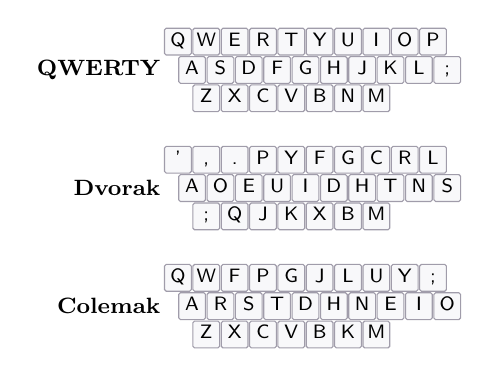
\begin{tikzpicture}
% Three keyboards stacked. Same 30 physical key positions; each layout
% reassigns the letters at those positions. Visual comparison highlights
% how a keymap is a re-binding of an unchanged physical substrate.
% Three keyboards stacked. Punctuation chars are wrapped in {} so
% TikZ's \foreach parser doesn't treat them as separators.
\foreach \layoutY/\name in {3.0/QWERTY, 1.5/Dvorak, 0.0/Colemak} {
  \node[anchor=east, font=\footnotesize\bfseries] at (-0.1, \layoutY+0.36) {\name};
}
% QWERTY rows
\foreach \l [count=\i] in {Q,W,E,R,T,Y,U,I,O,P}
  \node[kcap] at ({(\i-1)*0.36}, 3.72) {\strut\l};
\foreach \l [count=\i] in {A,S,D,F,G,H,J,K,L,{;}}
  \node[kcap] at ({(\i-1)*0.36+0.18}, 3.36) {\strut\l};
\foreach \l [count=\i] in {Z,X,C,V,B,N,M}
  \node[kcap] at ({(\i-1)*0.36+0.36}, 3.0) {\strut\l};
% Dvorak rows
\foreach \l [count=\i] in {{'},{,},{.},P,Y,F,G,C,R,L}
  \node[kcap] at ({(\i-1)*0.36}, 2.22) {\strut\l};
\foreach \l [count=\i] in {A,O,E,U,I,D,H,T,N,S}
  \node[kcap] at ({(\i-1)*0.36+0.18}, 1.86) {\strut\l};
\foreach \l [count=\i] in {{;},Q,J,K,X,B,M}
  \node[kcap] at ({(\i-1)*0.36+0.36}, 1.5) {\strut\l};
% Colemak rows
\foreach \l [count=\i] in {Q,W,F,P,G,J,L,U,Y,{;}}
  \node[kcap] at ({(\i-1)*0.36}, 0.72) {\strut\l};
\foreach \l [count=\i] in {A,R,S,T,D,H,N,E,I,O}
  \node[kcap] at ({(\i-1)*0.36+0.18}, 0.36) {\strut\l};
\foreach \l [count=\i] in {Z,X,C,V,B,K,M}
  \node[kcap] at ({(\i-1)*0.36+0.36}, 0) {\strut\l};
\end{tikzpicture}}
\caption{Three typing keymaps over the same physical substrate. Each layout is a re-binding of identical key positions to a different set of letters. QWERTY (Sholes 1873, never patented), Dvorak (Dvorak \& Dealey 1936, US 2{,}040{,}248), Colemak (Coleman 2006, public domain). The post-2010 fork ecosystem extends this line.}
\label{fig:typing-layouts}
\end{figure}

\section{Lineage II: Instrument Layouts}
\label{sec:lineage2}

Musical-instrument layouts have run a parallel history. Paul von Jankó's six-row isomorphic piano keyboard~\citep{janko1882} was endorsed by Liszt and Rubinstein, manufactured by Decker, Blüthner, and Bösendorfer, and taught at a Janko Conservatory in New York. By every social precondition for adoption it should have replaced the standard piano keyboard. It did not. Fewer than ten Janko pianos are known to survive. The Janko case is the negative pole of the keymap-as-social-software argument: every condition for propagation was met and propagation still failed. Whatever the social-software contract is, it is more than the sum of endorsements, manufacturers, and conservatories.

R.\ H.\ M.\ Bosanquet's generalized keyboard~\citep{bosanquet1875generalized} was a 53-equal-division-of-the-octave (53-EDO) enharmonic harmonium and a 1875 organ in 48-note schismatic and quarter-comma meantone, demonstrated to the South Kensington Museum in 1876. It is the ancestor of essentially every modern isomorphic controller. Kaspar Wicki patented an isomorphic note layout for bandoneon in 1896~\citep{wicki1896}; Brian Hayden, a concertina player, independently re-invented and re-patented essentially the same layout in 1986. The double invention by ninety years is itself an argument: the layout has the character of a \emph{discovery}, the kind of object that recurs because the underlying structure of music makes it useful, not because it is a unique cultural artifact.

\begin{figure}[t]
\centering
\resizebox{0.88\columnwidth}{!}{%
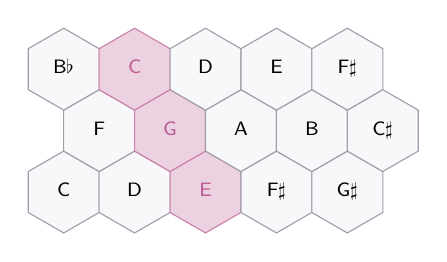
\begin{tikzpicture}
% Compact Wicki-Hayden-style hex schematic. Same-row neighbors
% differ by a whole tone; up-and-right neighbors differ by a P4.
% C major triad (C-E-G) highlighted; the same shape transposes to
% any key by translation across the surface ("isomorphism" claim).
% Hexes are EXPLICIT PATHS, not regular-polygon nodes — TikZ node
% sizing breaks the lattice. Pointy-top hexagon, circumradius R:
% width = sqrt(3)R, height = 2R. Tessellation: horizontal pitch =
% sqrt(3)R, row step = 1.5R, odd-row offset = sqrt(3)R/2.
\def\R{0.52}
\def\hexn#1#2#3{\begin{scope}[shift={(#1,#2)}]
  \draw[keystroke, fill=keyfill]
    (30:\R) -- (90:\R) -- (150:\R) -- (210:\R) -- (270:\R) -- (330:\R) -- cycle;
  \node[font=\scriptsize\sffamily, inner sep=0pt] at (0,0) {\strut#3};
\end{scope}}
\def\hexm#1#2#3{\begin{scope}[shift={(#1,#2)}]
  \draw[keymapped!70, fill=keymapped!25]
    (30:\R) -- (90:\R) -- (150:\R) -- (210:\R) -- (270:\R) -- (330:\R) -- cycle;
  \node[font=\scriptsize\sffamily, text=keymapped!90, inner sep=0pt] at (0,0) {\strut#3};
\end{scope}}
\def\hp{0.9006}    % horizontal pitch (sqrt(3) * R)
\def\vp{0.78}      % vertical pitch (1.5 * R)
\def\offx{0.4503}  % horizontal offset for alternate rows (hp / 2)
% Row 0 (bottom)
\hexn{0}{0}{C}
\hexn{\hp}{0}{D}
\hexm{2*\hp}{0}{E}
\hexn{3*\hp}{0}{F$\sharp$}
\hexn{4*\hp}{0}{G$\sharp$}
% Row 1 (middle, offset)
\hexn{\offx}{\vp}{F}
\hexm{\offx + \hp}{\vp}{G}
\hexn{\offx + 2*\hp}{\vp}{A}
\hexn{\offx + 3*\hp}{\vp}{B}
\hexn{\offx + 4*\hp}{\vp}{C$\sharp$}
% Row 2 (top)
\hexn{0}{2*\vp}{B$\flat$}
\hexm{\hp}{2*\vp}{C}
\hexn{2*\hp}{2*\vp}{D}
\hexn{3*\hp}{2*\vp}{E}
\hexn{4*\hp}{2*\vp}{F$\sharp$}
\end{tikzpicture}}
\caption{Wicki--Hayden hex layout (Wicki 1896 / Hayden 1986). Same-row neighbors differ by a whole tone; up-and-right neighbors by a perfect fourth. The C major triad ($C\,E\,G$) is highlighted: the chord is a fixed three-cell shape on the surface, and translating that shape transposes the chord to any key. ``Transposition is translation'' is the central isomorphic-keyboard claim, and the property the standard piano's white-and-black asymmetry sacrifices.}
\label{fig:wicki}
\end{figure}

\begin{figure}[t]
\centering
% Four structural diagrams in the paper's abstract idiom (strings as
% lines, valves as interval nodes, holes as a graded constellation) —
% chosen over photographic/illustrative treatments.
\resizebox{\columnwidth}{!}{%
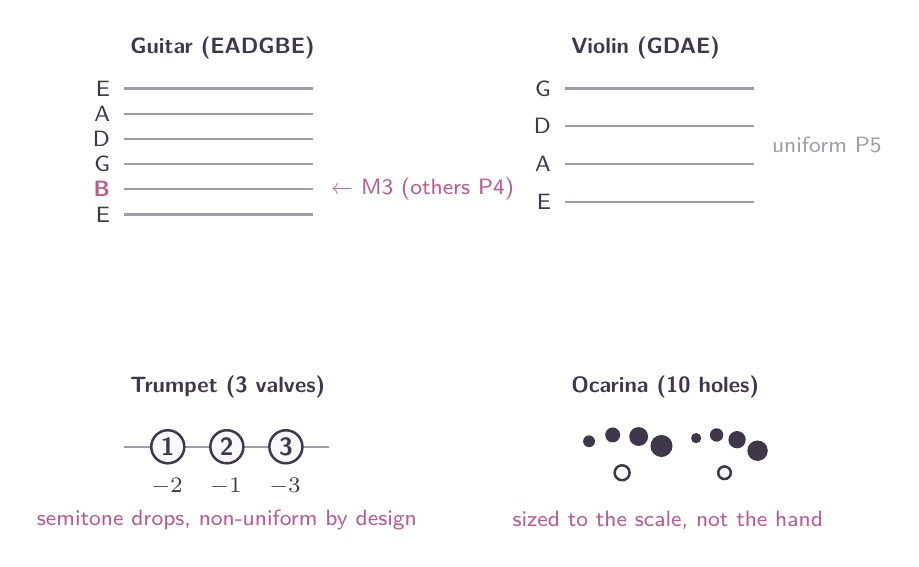
\begin{tikzpicture}[
  string/.style={draw=keystroke, line width=0.8pt},
  ilabel/.style={font=\footnotesize\sffamily\bfseries, text=acdark}
]
% Guitar (top left): 6 strings, M3 break flagged in pink
\begin{scope}[shift={(0, 0)}]
  \node[ilabel, anchor=south west] at (-0.05, 1.95) {Guitar (EADGBE)};
  \foreach \i/\note/\hl in {1/E/0, 2/A/0, 3/D/0, 4/G/0, 5/B/1, 6/E/0} {
    \draw[string] (0, {1.70 - (\i-1)*0.32}) -- (2.4, {1.70 - (\i-1)*0.32});
    \ifnum\hl=1
      \node[font=\footnotesize\sffamily\bfseries, text=keymapped!90, anchor=east]
        at (-0.06, {1.70 - (\i-1)*0.32}) {\note};
    \else
      \node[font=\footnotesize\sffamily, text=acdark, anchor=east]
        at (-0.06, {1.70 - (\i-1)*0.32}) {\note};
    \fi
  }
  \node[font=\footnotesize\sffamily, text=keymapped!90, anchor=west]
    at (2.5, 0.42) {$\leftarrow$ M3 (others P4)};
\end{scope}
% Violin (top right): 4 strings, uniform P5
\begin{scope}[shift={(5.6, 0)}]
  \node[ilabel, anchor=south west] at (-0.05, 1.95) {Violin (GDAE)};
  \foreach \i/\note in {1/G, 2/D, 3/A, 4/E} {
    \draw[string] (0, {1.70 - (\i-1)*0.48}) -- (2.4, {1.70 - (\i-1)*0.48});
    \node[font=\footnotesize\sffamily, text=acdark, anchor=east]
      at (-0.06, {1.70 - (\i-1)*0.48}) {\note};
  }
  \node[font=\footnotesize\sffamily, text=keystroke, anchor=west]
    at (2.5, 0.98) {uniform P5};
\end{scope}
% Trumpet (bottom left): the three valves as interval nodes on the
% air path; each lowers pitch by a DIFFERENT interval.
\begin{scope}[shift={(0, -3.2)}]
  \node[ilabel, anchor=south west] at (-0.05, 0.85) {Trumpet (3 valves)};
  \draw[keystroke, line width=0.8pt] (0, 0.35) -- (2.6, 0.35);
  \foreach \x/\n/\offs in {0.55/1/$-2$, 1.30/2/$-1$, 2.05/3/$-3$} {
    \draw[acdark, fill=keyfill, line width=0.9pt] (\x, 0.35) circle (0.21);
    \node[font=\small\sffamily\bfseries, text=acdark] at (\x, 0.35) {\n};
    \node[font=\footnotesize\sffamily, text=acdark] at (\x, -0.14) {\offs};
  }
  \node[font=\footnotesize\sffamily, text=keymapped!90]
    at (1.3, -0.58) {semitone drops, non-uniform by design};
\end{scope}
% Ocarina (bottom right): the bare hole constellation, radii graded
% to pitch, clustered asymmetrically (Donati 1853). Filled = finger,
% outlined = thumb.
\begin{scope}[shift={(5.6, -3.2)}]
  \node[ilabel, anchor=south west] at (-0.05, 0.85) {Ocarina (10 holes)};
  \fill[acdark] (0.30, 0.42) circle (0.075);
  \fill[acdark] (0.60, 0.50) circle (0.095);
  \fill[acdark] (0.93, 0.48) circle (0.120);
  \fill[acdark] (1.22, 0.36) circle (0.140);
  \fill[acdark] (1.66, 0.46) circle (0.065);
  \fill[acdark] (1.92, 0.50) circle (0.085);
  \fill[acdark] (2.18, 0.44) circle (0.110);
  \fill[acdark] (2.44, 0.30) circle (0.130);
  \draw[acdark, line width=0.9pt] (0.72, 0.02) circle (0.095);
  \draw[acdark, line width=0.9pt] (2.02, 0.02) circle (0.080);
  \node[font=\footnotesize\sffamily, text=keymapped!90]
    at (1.3, -0.58) {sized to the scale, not the hand};
\end{scope}
\end{tikzpicture}}
\caption{Four asymmetric pitch interfaces. Guitar EADGBE is uniform in perfect fourths \emph{except} the major-third between G and B (the irregularity that lets the standard chord shapes lie under the hand, and that the literature of folk, blues, jazz, and rock guitar has been authored against). Violin keeps strict P5s but each open string is a different absolute pitch. The trumpet's three valves lower pitch by two, one, and three semitones --- deliberately non-uniform so combinations reach the chromatic set. The ocarina's ten finger holes are sized and clustered to the scale rather than the hand (Donati's 1853 standardization at Budrio). The standard piano belongs to the same family: the diatonic naming keymap embodied in many surfaces, each with its own asymmetry.}
\label{fig:asymmetric-instruments}
\end{figure}

Each of these surfaces carries its own genealogy. The three-valve trumpet (Stölzel and Blühmel, c.\ 1814) standardized after a century of natural-trumpet practice, with Vienna and rotary valve variants each constituting its own keymap-over-pitch. The ocarina runs from Mesoamerican vessel flutes through Giuseppe Donati's 1853 standardization at Budrio, where asymmetric finger-hole placement made the 10-hole pattern teachable. The guitar's EADGBE tuning crystallized in the 1700s out of lute tunings: the B-string irregularity breaks the otherwise-uniform fourths so the open chord shapes lie under the hand, and the entire literature of folk, blues, jazz, and rock guitar has been authored against that single irregular interval. The violin's strict perfect fifths (G\,D\,A\,E) anchor the fifths-based string-section conventions the orchestral repertoire is written into. In every case the asymmetry is not a flaw the music tolerates but an inheritance the music has been authored around --- it determines what a beginner learns first, what a practice exercise looks like, what notation traveled. The standard piano keyboard sits inside this tradition, not above it; the isomorphic alternatives propose something more radical than they sometimes admit, which is the dissolution of the keymap-of-pitch-naming that connects all of these instrument families to one another.

The standard reading of Jankó's failure --- and the marginality of the Wicki--Hayden / hex-grid family more broadly --- is path-dependence on the David--Liebowitz model: the piano persists by lock-in alone. A harder reading is available. The white-and-black asymmetry of the standard piano keyboard is a chromatic-circle landmark map --- the player knows where $C$ is because it sits left of two blacks --- offloading absolute pitch position from memory to the eye and the hand. Strip the asymmetry and the offloaded information has nowhere to land: transposition becomes translation, but absolute location becomes recall. Four centuries of repertoire have absorbed the asymmetry into \emph{key character} --- the fingering of $F^\sharp$ major differs from that of $C$ major, and the music has been written to that differing --- so removing the ``accident of history'' flattens an axis of meaning the literature has been authored along. This does not dissolve the path-dependence story so much as cut along it from the other side: the piano is path-dependent \emph{and} the path has produced an object not strictly equivalent to its alternatives. The deeper move is to treat the Western tonal system itself as a keymap: the seven-letter diatonic naming $C\,D\,E\,F\,G\,A\,B$ is already a social-software contract over pitch space, written into theory, pedagogy, and every key signature. The piano's white keys are the physical realization of that keymap; the black keys are the alterations notation already names with $\sharp$ and $\flat$. The standard piano is thus doing two jobs at once --- physical interface and notational encoding --- and the isomorphic alternatives propose to dissolve the second to optimize the first. The argument is scoped to the 12-tone-equal-tempered repertoire that names pitches with the diatonic letters; outside it --- xenharmonic music in 19-, 22-, 31-, 53-EDO, Maqam and other tonal systems with different pitch-naming keymaps --- the piano is actively obstructive and the isomorphic line from Bosanquet through the Lumatone has a strong, repertoire-grounded claim. Within that scope, the same keymap-of-pitch-naming is what \texttt{notepat} (\textsection\ref{sec:notepat}) preserves, carried onto QWERTY's letter caps, where pressing the letter \texttt{C} plays the note $C$. Where Jankó dissolves the naming keymap to optimize the physical interface, and the chromatic-staircase DAW convention dissolves \emph{both} (\textsection\ref{sec:daw}), \texttt{notepat} keeps the naming contract unchanged and re-asks only the question Sholes' 1873 mechanics asked: what physical surface should carry it forward.

The contemporary descendants are commercial products: the C-Thru AXiS-49 (2008)~\citep{cthru2008axis49}, Jim Plamondon's Thummer~\citep{plamondon2003thummer}, the Roger Linn LinnStrument, the ROLI Seaboard, the Lumatone hex grid, and Lippold Haken's Continuum Fingerboard~\citep{haken1998indiscrete}. Andrew Milne, William Sethares, and James Plamondon's papers on isomorphic controllers and tuning continua~\citep{milne2007isomorphic,milne2008tuning} provide the theoretical foundation. What is striking from a keymap-as-social-software view is that these instruments \emph{ship configurable}: the layout is an explicit object the user uploads, and the xenharmonic community shares layouts as files. The Lumatone in particular treats the keymap as the unit of distribution. The instrument is a substrate; the keymap is the artifact that makes it musical.

\section{The DAW Chromatic-Staircase: Convergence Without Ownership}
\label{sec:daw}

The strongest contemporary case for the keymap-as-social-software argument is the de-facto chromatic-staircase QWERTY-piano keymap shared by every major digital audio workstation. Ableton Live, Logic Pro, GarageBand, and FL Studio all ship the same convention by default~\citep{ableton_musical_typing,apple_logic_musicaltyping,imageline_typing_piano}. The shape of the convention is: take the lower three rows of the QWERTY keyboard; treat one row as the white keys of a chromatic scale, ascending from C; and treat the row above as the black keys, in the gaps where black keys would fall on a piano. Ableton, Logic, and GarageBand use \keys{A,S,D,F,G,H,J,K} (home row) for the white keys $C\,D\,E\,F\,G\,A\,B\,C$ and \keys{W,E,T,Y,U} (row above) for the black keys $C^\sharp\,D^\sharp\,F^\sharp\,G^\sharp\,A^\sharp$. FL Studio uses the bottom row \keys{Z,X,C,V,B,N,M} for the lower octave's white keys and the same row-above pattern for the black keys. The principle is identical. The exact row assignment differs by one row.

No one designed this convention. No spec defines it. There is no governing body, no maintainer, no funding mechanism. The convention exists because the four implementations agree, and the four implementations agree because the convention was already present in the 1990s tracker software that preceded the modern DAW (FastTracker, Renoise, Impulse Tracker), and because every user who has learned one DAW expects the next to behave the same. Tutorial documentation written for one DAW transfers, more or less, to another. This is the \emph{social-software contract} in its purest form: a versioned virtual object that propagates through pedagogy and expectation, with no central authority.

\begin{figure}[t]
\centering
\resizebox{\columnwidth}{!}{%
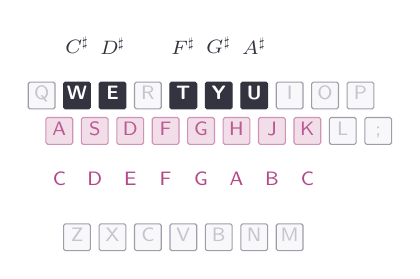
\begin{tikzpicture}
% Upper QWERTY row (sharps in DAW chromatic-staircase). Only 5 keys
% are mapped (W E T Y U); R and I sit in the gaps with no note.
\foreach \l/\note/\mapped [count=\i] in {%
  Q/{}/0, W/$C^\sharp$/1, E/$D^\sharp$/1, R/{}/0, T/$F^\sharp$/1,
  Y/$G^\sharp$/1, U/$A^\sharp$/1, I/{}/0, O/{}/0, P/{}/0%
}{
  \ifnum\mapped=1
    \node[kcap sharp] (k\i) at ({(\i-1)*0.45}, 1.8) {\strut\l};
    \node[font=\scriptsize\sffamily, text=keysharp, anchor=south]
      at ({(\i-1)*0.45}, 2.2) {\note};
  \else
    \node[kcap, text=keystroke!60] (k\i) at ({(\i-1)*0.45}, 1.8) {\strut\l};
  \fi
}
% Home row (whites). 8 of 10 keys mapped (A through K = C..C).
\foreach \l/\note/\mapped [count=\i] in {%
  A/C/1, S/D/1, D/E/1, F/F/1, G/G/1, H/A/1, J/B/1, K/C/1, L/{}/0, {;}/{}/0%
}{
  \ifnum\mapped=1
    \node[kcap mapped] at ({(\i-1)*0.45+0.225}, 1.35) {\strut\l};
    \node[font=\scriptsize\sffamily, text=keymapped, anchor=north]
      at ({(\i-1)*0.45+0.225}, 0.95) {\note};
  \else
    \node[kcap, text=keystroke!60] at ({(\i-1)*0.45+0.225}, 1.35) {\strut\l};
  \fi
}
% Bottom row — unmapped in the home-row variant; FL Studio uses it
% for whites, but at this scale the comparison stays clean.
\foreach \l [count=\i] in {Z,X,C,V,B,N,M}
  \node[kcap, text=keystroke!60] at ({(\i-1)*0.45+0.45}, 0.0) {\strut\l};
\end{tikzpicture}}
\caption{The DAW chromatic-staircase QWERTY-piano keymap (Ableton, Logic, GarageBand variant). Home row \texttt{A~S~D~F~G~H~J~K} plays the white keys $C$ through $C$; the row above places sharps in the gaps where the piano black keys would fall ($C^\sharp\,D^\sharp$ then a gap at \texttt{R}, $F^\sharp\,G^\sharp\,A^\sharp$, then gaps). The QWERTY letter on each cap bears no relation to the note name it produces.}
\label{fig:daw-staircase}
\end{figure}

It is also, I will argue, badly designed. The chromatic-staircase keymap has three structural weaknesses. \textbf{First}, the QWERTY letter on each key bears no relation to the note name it produces. \key{A} plays C; \key{S} plays D; \key{D} plays E (Figure~\ref{fig:daw-staircase}). A user who has learned the Western seven-note scale gains no purchase on the keymap from that knowledge. \textbf{Second}, the keymap is monohanded by default --- the entire usable range sits on the left side of the keyboard, with the right hand idle. \textbf{Third}, the keymap is illegible without a tutorial: there is no mnemonic, no diagram printed on the physical keys, and no way to derive the mapping from first principles. A keymap that requires a manual is a keymap that has lost its social-software character.

A useful contrast is the \emph{WASD} convention in PC gaming. WASD has the same structural shape as the chromatic-staircase --- an unowned, unspecified, cross-application user-input convention --- but a different propagation history. Pre-WASD, PC games defaulted to arrow keys (Wolfenstein 3D, Doom, the Quake series through 1997)~\citep{wikipedia_arrow_keys}; intermediate experiments included System Shock's ASDX (1994) and Descent's AZ+QE. Dennis ``Thresh'' Fong, a competitive Quake player, popularized the WASD layout through his self-published configuration guide~\citep{thresh_quake_bible} and won the first nationwide Quake tournament in 1997. Valve's Half-Life shipped WASD as default in 1998, and by the early 2000s the convention had saturated PC games~\citep{fenlon2016wasd}. WASD persists for a reason the DAW chromatic-staircase does not: it is genuinely better than the official default. It frees the right hand for the mouse, sits adjacent to Shift / Space / Ctrl / Tab, and exploits home-row finger placement on a QWERTY keyboard. The structural lesson is that propagation is a function of social mediation \emph{and} fitness: WASD propagated because Fong's pedagogy reached players \emph{and} the mapping won on the merits. The chromatic-staircase propagated through pedagogy alone, despite the merits running the other way. Both cases sit in the same category --- unowned conventions that govern user input across applications. They demonstrate that the category is large enough to span both the well-designed and the badly-designed, the user-validated and the inherited-by-inertia.

\section{Notepat: Notes That Name Themselves}
\label{sec:notepat}

Against this incumbent, \texttt{notepat} proposes a different keymap (Figure~\ref{fig:notepat-keymap}). The design principle is single: \emph{notes that name themselves}. The QWERTY letter \key{C} plays C. The QWERTY letter \key{D} plays D. The seven naturals of the Western scale --- $C\,D\,E\,F\,G\,A\,B$ --- play the notes their letters name. The upper octave continues alphabetically: \keys{H,I,J,K,L,M,N} for $C_5\,D_5\,E_5\,F_5\,G_5\,A_5\,B_5$. Sharps sit one row above their natural, by analogy to the black keys of a piano, where the QWERTY letters allow it: \keys{V,S,W,R,Q} for $C^\sharp\,D^\sharp\,F^\sharp\,G^\sharp\,A^\sharp$. The lower octave falls under the left hand; the upper octave falls under the right.

The keymap reverses each of the chromatic-staircase's three weaknesses. \textbf{First}, the letter on each key \emph{is} the note name. Anyone who knows the Western scale already knows the keymap. \textbf{Second}, the layout is two-handed by default: the left hand plays the lower octave; the right hand mirrors it on the upper. \textbf{Third}, the keymap is self-documenting: the diagram in Figure~\ref{fig:notepat-keymap} can be reproduced from memory by anyone who can spell ``CDEFGAB.''

\texttt{notepat}'s contribution is not the implementation. The implementation is, by design, modest: a few hundred lines of JavaScript routing keyboard events to an audio synthesis API. The contribution is the keymap. \texttt{notepat} is presented across six implementations --- the web piece at \texttt{notepat.com}, the AC Native bare-metal port, the MenuBand macOS menubar app, the AC-Notepat Max for Live device, the Remote phone app, and a VST3 scaffold --- and the keymap is the one thing that is identical across all of them. It is the \texttt{notepat}-shaped social-software contract.

A reader comparing the implementations side by side will notice keys doing things beyond the table in Figure~\ref{fig:notepat-keymap}. On AC Native and MenuBand, holding \texttt{Space} reverse-plays the last several seconds of actual audio output. On the web piece and AC Native, holding \texttt{Shift} while striking a note gives that voice a long decay tail when released; holding \texttt{Enter} holds the voice indefinitely, and \texttt{Backspace} clears every held voice. On MenuBand and AC Native, \texttt{Control}, \texttt{Alt}, and the two together promote a single keypress to a major, minor, or suspended triad. None of this appears in the keymap diagram, and the omission is deliberate. These bindings form an \emph{extended performance layer}, and the line between that layer and the tonal mapping is the boundary of the social-software contract itself (Table~\ref{tab:contract-line}).

\begin{table}[t]
\footnotesize
\setlength{\tabcolsep}{3pt}
\renewcommand{\arraystretch}{1.05}
\centering
\caption{The \texttt{notepat} bindings, divided at the contract line. Above the line: the tonal mapping, identical across all implementations --- the social-software object. Below it: the extended performance layer, where each substrate is free to differ.}
\label{tab:contract-line}
\begin{tabularx}{\columnwidth}{@{}>{\RaggedRight}p{0.30\columnwidth}>{\RaggedRight}X>{\RaggedRight\arraybackslash}p{0.21\columnwidth}@{}}
\toprule
\textbf{Binding} & \textbf{Meaning} & \textbf{Where} \\
\midrule
\multicolumn{3}{@{}l}{\emph{Tonal contract}} \\[0.1em]
\texttt{C D E F G A B} & naturals $C_4$--$B_4$, left hand & all \\
\texttt{H I J K L M N} & naturals $C_5$--$B_5$, right hand & all \\
\texttt{V S W R Q} & sharps, one row above & all \\
\midrule
\multicolumn{3}{@{}l}{\emph{Extended performance layer}} \\[0.1em]
\texttt{Shift} (hold) & sustain: long decay tail & web, Native \\
\texttt{Enter} (hold) & hold voice; \texttt{Backspace} clears & web, Native \\
\texttt{Space} (hold) & reverse-play recent audio & Native, MenuBand \\
\texttt{Ctrl}\,/\,\texttt{Alt}\,/\,both & major\,/\,minor\,/\,sus2 triad & MenuBand, Native \\
\texttt{<}~\texttt{>} & per-hand octave shift & web \\
\bottomrule
\end{tabularx}
\end{table}

The two halves of Table~\ref{tab:contract-line} are governed by different rules. Above the line, deviation is breakage: an implementation that remapped \texttt{C} away from the note $C$ would not be a \texttt{notepat} port but a different instrument. Below the line, deviation is idiom: each substrate grows the gestures its body affords. The bare-metal OS, owning the whole machine, can ring-buffer its own audio output and play it backwards; the menubar app, riding a system-wide event tap, leans on modifier chords; the web piece, living in a browser tab, sustains and holds. Users do not experience these differences as breakage, and no implementation is obliged to carry another's gestures. The same two-tier structure is visible in the older cases: QWERTY-the-contract says nothing about media keys or \texttt{Fn} layers, which vary freely by vendor without anyone calling a ThinkPad a fork of QWERTY; Vim's core motions are contract while plugin bindings are idiom. A keymap, this suggests, is not the set of all bindings an implementation ships. It is the subset whose alteration the community would experience as a breach of identity --- and one practical test for which side of the line a binding falls on is whether the notation surface (\textsection\ref{sec:notation}) carries it. \texttt{C D E F G A B} travels as text; ``hold space to reverse time'' is a per-substrate gesture that must be re-taught, by demonstration, at every port.

This is the move the paper is asking the reader to see. The dominant DAW chromatic-staircase keymap was never \emph{chosen} --- it was \emph{inherited} from tracker software, persisted by user expectation, and locked in by cross-application convention. \texttt{notepat} demonstrates that the gap is open: that a deliberately-designed alternative can be authored by a single developer in a few hundred lines of code, shipped across multiple implementations in a year, and offered to a wider community as a competing social-software contract. The political stake is small in any one instance and large in aggregate: \emph{the gap is open everywhere}.

\section{Notation: The Discursive Surface}
\label{sec:notation}

The argument so far has treated the keymap as a table. But a keymap is not only a table. It also has a \emph{notation} --- a textual form in which usage of the keymap is read, written, taught, cited, and argued over. The notation is the discursive surface of the keymap. It is also, I will argue, the half of the keymap that actually travels. A keymap whose notation is portable propagates as text; a keymap whose notation is awkward or absent propagates only as muscle memory. The quality of the notation is therefore a designable property of the keymap, not a derivative artifact. A designer who ships only the binding-table has shipped half of the object.

The canonical case is Vim. Vim's underlying keymap is a table mapping keystrokes to editor commands: \texttt{d} initiates a delete operator, \texttt{i} an inner text-object, \texttt{w} a word motion. What travels in Vim discourse, however, is not the table. What travels is a \emph{notation}: \texttt{dd}, \texttt{ciw}, \texttt{gg}, \texttt{:wq}, \texttt{<C-w>} (Figure~\ref{fig:vim-modes}). Tutorials, blog posts, README files, vimtutor, and the long-running vim-vs-emacs argument are all conducted in this notation. The notation is so portable that it survives outside Vim entirely: \emph{vim mode} appears in Visual Studio Code, in JupyterLab, in shells via \texttt{set -o vi}, in macOS Cocoa text fields, in browsers via Vimium. What is being ported is the notation. The runtime is contingent.

\begin{figure}[t]
\centering
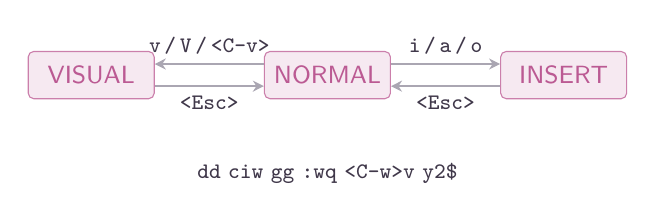
\begin{tikzpicture}[
  modebox/.style={draw=keymapped!70, fill=keymapped!12,
                   rounded corners=2pt, minimum width=1.6cm,
                   minimum height=0.6cm, font=\small\sffamily,
                   text=keymapped!90, inner sep=2pt},
  arrow/.style={-{Stealth[length=4pt,width=4pt]}, draw=keystroke!90,
                 line width=0.5pt},
  cmd/.style={font=\footnotesize\ttfamily, text=acdark}
]
% Three Vim modes wired by their command-notation transitions.
\node[modebox] (normal) at (0, 0) {NORMAL};
\node[modebox] (insert) at (3.0, 0) {INSERT};
\node[modebox] (visual) at (-3.0, 0) {VISUAL};
\draw[arrow] ([yshift=4pt]normal.east) -- node[above, cmd] {\texttt{i}\,/\,\texttt{a}\,/\,\texttt{o}} ([yshift=4pt]insert.west);
\draw[arrow] ([yshift=-4pt]insert.west) -- node[below, cmd] {\texttt{<Esc>}} ([yshift=-4pt]normal.east);
\draw[arrow] ([yshift=4pt]normal.west) -- node[above, cmd] {\texttt{v}\,/\,\texttt{V}\,/\,\texttt{<C-v>}} ([yshift=4pt]visual.east);
\draw[arrow] ([yshift=-4pt]visual.east) -- node[below, cmd] {\texttt{<Esc>}} ([yshift=-4pt]normal.west);
% A row of canonical commands underneath
\node[font=\footnotesize\ttfamily, text=acdark, anchor=north] at (0, -1.0)
  {\texttt{dd}\,\,\texttt{ciw}\,\,\texttt{gg}\,\,\texttt{:wq}\,\,\texttt{<C-w>v}\,\,\texttt{y2}\$};
\end{tikzpicture}
\caption{Vim's modal keymap and its travelling notation. Modes (NORMAL, INSERT, VISUAL) are connected by labeled keystroke transitions; common commands (\texttt{dd} delete-line, \texttt{ciw} change-inner-word, \texttt{gg} go-top, \texttt{:wq} write-and-quit, etc.) are the discursive currency of the keymap. The notation is so portable it has been re-implemented in VS~Code, JupyterLab, Vimium, the macOS Cocoa text system, and \texttt{set -o vi}.}
\label{fig:vim-modes}
\end{figure}

The DAW chromatic-staircase is the negative case. There is no portable notation for it. Writing a melody played on Ableton's musical typing requires falling back to event-sequence prose --- ``press \key{A}, then \key{S}, then \key{D}'' --- which describes input rather than music. Compare to Singmaster cube notation~\citep{singmaster1981notes} (Figure~\ref{fig:singmaster}), where \texttt{R U R' U' R U2 R'} lets a Rubik's-cube algorithm travel intact between cubers; or to the Nashville Number System~\citep{matthews1984nashville,williams1988nashville}, where ``1--4--5'' lets a chord progression travel between session musicians; or to Plover steno theory~\citep{knight2010plover}, where the chord notation lets stenographic patterns travel through a community-edited dictionary. The DAW staircase has no such handle. Its keys are addressable only by their physical position. The keymap therefore exists in muscle memory and rarely on the page --- which is exactly why it has lower discursive presence than Vim despite an arguably larger user base.

\begin{figure}[t]
\centering
\resizebox{0.62\columnwidth}{!}{%
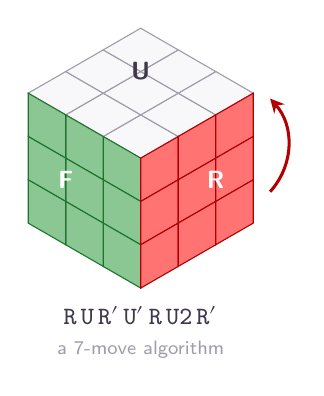
\begin{tikzpicture}
% Isometric Rubik's cube, three visible faces: U (top), F (front-
% left), R (right). Faces are explicit-path parallelogram grids built
% from iso axes er=(0.866,0.5)s (right-up), el=(-0.866,0.5)s
% (left-up), ed=(0,-1)s (down), all meeting at the shared front-top
% vertex at the origin. The R face is tinted with a quarter-turn
% arrow: the diagram shows the first move of the algorithm below.
\def\s{0.55}
% Top face U: cells spanned by er and el
\foreach \i in {0,1,2} \foreach \j in {0,1,2}
  \draw[keystroke, fill=keyfill]
    ({0.866*\s*(\i-\j)}, {0.5*\s*(\i+\j)})
    -- ++({0.866*\s}, {0.5*\s})
    -- ++({-0.866*\s}, {0.5*\s})
    -- ++({-0.866*\s}, {-0.5*\s}) -- cycle;
% Front-left face F: cells spanned by el and ed — green stickers
\foreach \i in {0,1,2} \foreach \j in {0,1,2}
  \draw[acgreen!75!black, fill=acgreen!55]
    ({-0.866*\s*\i}, {0.5*\s*\i - \s*\j})
    -- ++({-0.866*\s}, {0.5*\s})
    -- ++(0, {-\s})
    -- ++({0.866*\s}, {-0.5*\s}) -- cycle;
% Right face R: cells spanned by er and ed — red stickers (mid-turn)
\foreach \i in {0,1,2} \foreach \j in {0,1,2}
  \draw[red!70!black, fill=red!55]
    ({0.866*\s*\i}, {0.5*\s*\i - \s*\j})
    -- ++({0.866*\s}, {0.5*\s})
    -- ++(0, {-\s})
    -- ++({-0.866*\s}, {-0.5*\s}) -- cycle;
% Face labels at face centers — standard sticker scheme:
% white up, green front, red right.
\node[font=\small\sffamily\bfseries, text=acdark]
  at (0, {1.5*\s + 0.5*\s}) {U};
\node[font=\small\sffamily\bfseries, text=white]
  at ({-0.866*\s*1.5 - 0.433*\s}, {0.75*\s - 1.5*\s + 0.25*\s}) {F};
\node[font=\small\sffamily\bfseries, text=white]
  at ({0.866*\s*1.5 + 0.433*\s}, {0.75*\s - 1.5*\s + 0.25*\s}) {R};
% Quarter-turn arrow for R: curved arrow hugging the right face's
% outer edge, pointing upward (clockwise as seen from the right).
\draw[-{Stealth[length=5pt,width=5pt]}, line width=1.1pt, red!70!black]
  ({0.866*\s*3.45}, {0.5*\s*3.45 - 2.5*\s})
  to[bend right=42]
  ({0.866*\s*3.45}, {0.5*\s*3.45 - 0.35*\s});
% Notation row underneath
\node[font=\small\ttfamily, anchor=north, text=acdark]
  at (0, {-3.2*\s}) {R\,U\,R$'$\,U$'$\,R\,U2\,R$'$};
\node[font=\scriptsize\sffamily, anchor=north, text=keystroke]
  at (0, {-4.0*\s}) {a 7-move algorithm};
\end{tikzpicture}}
\caption{Singmaster's cube notation~\citep{singmaster1981notes}. Each capital letter names a face (\textsf{U}p, \textsf{D}own, \textsf{L}eft, \textsf{R}ight, \textsf{F}ront, \textsf{B}ack); a bare letter is a clockwise quarter-turn, a primed letter ($\,'$) a counter-clockwise quarter-turn, and a digit-2 a half-turn. The seven-token string \texttt{R U R$'$ U$'$ R U2 R$'$} is a complete algorithm portable between cubers, GitHub repos, and YouTube tutorials --- the keymap-notation pair traveling as text. Faces carry the standard sticker scheme (white up, green front, red right); \textsf{R} is drawn mid-quarter-turn: the algorithm's first move.}
\label{fig:singmaster}
\end{figure}

\texttt{notepat}'s ``notes-name-themselves'' design has, as a structural side-effect, a notation that costs nothing to learn. To write a notepat sequence, one writes \texttt{C D E F G A B} --- which is also standard music notation. The notation is not invented for \texttt{notepat}; it is \emph{inherited} from an existing literacy. A pianist who has never seen a notepat keymap can read a notepat score; conversely, a notepat performer who learns the keymap is also rehearsing standard pitch-letter literacy. This is what a well-designed notation surface looks like: the notation is so trivially derivable from prior knowledge that learning the notation costs nothing. Ableton's chromatic-staircase, in contrast, would require a notepat-like score to be re-coded as \texttt{A S D F G H J} --- a private notation tethered to one keymap, useful nowhere else.

The empirical literature on keyboard shortcut adoption supports this reading. Peres et al.\ found that working alongside other shortcut users is a stronger predictor of shortcut use than computer experience alone~\citep{peres2004shortcut}. Lozhkina et al.\ extend the result: the discovery channel for shortcuts is interpersonal and visual~\citep{lozhkina2025discovery}. Wang et al.\ explicitly use the term \emph{vocabulary} to name what shortcut design hands a user~\citep{wang2020keymap}. The argument of this paper sharpens those findings: the social mediation is not a generic effect of being-around-other-users; it is a specific transmission via the notation surface. Colleagues read each other's screens, see \texttt{:wq}, ask, learn. Where there is no transmissible notation, there is no social mediation to mediate. The same logic explains the success of live-coding mini-notations: Alex McLean and Geraint Wiggins's TidalCycles pattern language~\citep{mclean2010tidal}, ported to JavaScript as Strudel~\citep{roos2023strudel}, and Olivia Jack's Hydra transform-chains for live-coded visuals~\citep{jack2018hydra}, alongside ABC notation for folk music~\citep{walshaw_abc}. In each case the runtime is contingent --- Haskell, JavaScript, WebGL, MIDI players --- but the notation carries the practice across runtimes, workshops, and decades.

The corollary catalog of \textsection\ref{sec:corollaries} is, when read through this lens, almost entirely a catalog of notations. Singmaster, Nashville, ABC, IPA, Camelot, fighting-game numpad notation, scientific pitch, the NATO spelling alphabet, knitting abbreviations --- each is a notation derived from a keymap (or input mapping) that allowed the underlying practice to travel as text. The keymap-notation pair is the unit. The keymap supplies the affordance; the notation supplies the propagation surface.

The structural claim has a deeper diagnostic. Walter Ong's distinction between orality and literacy~\citep{ong1982orality}, building on Havelock's account of the same transition in ancient Greece~\citep{havelock1963preface}, cuts the question cleanly. \emph{Oral} traditions persist through performance, person-to-person transmission, and repeated approximation; they have no canonical text, mutate slightly across instances, and survive because performers keep performing them. \emph{Literate} traditions persist through fixed text, authoritative editions, and exact reproduction; they have specs, canons, and reference implementations. The standard frames of computing scholarship are all literate frames: an open-source license governs a fixed text, a protocol governs a fixed wire format, a format governs a fixed encoding. The DAW chromatic-staircase is a primary-oral keymap --- there is no canonical text, only four implementations that agree by performance. Vim has both an oral substrate (one learns the keymap by watching another developer's screen) and a literate edge (the notation: \texttt{:wq}, \texttt{<C-w>}, \texttt{ciw}). \texttt{notepat} collapses the literate side into the standing literacy of pitch-letter notation: the keymap inherits its written form from a centuries-older literate practice. The oral substrate is the keymap; the notation is the literate fixation; where the latter succeeds, the former gains a body that travels. The orality-literacy axis is the diagnosis of why keymaps escape the open-source/proprietary frame at all: the standard frames are literate frames, but the keymap is at least partly oral, and the absence of a literate fixation in academic and industrial discourse alike is the symptom that gave this paper its motivating question.

The same orality-literacy axis explains a feature of the keymap literature: there isn't much of one. The PC Gamer history of WASD~\citep{fenlon2016wasd} is the canonical popular-press source on a convention that controls hundreds of millions of hours of gameplay; the equivalent academic literature is essentially empty. That is not because keymaps are unimportant. It is because the existing apparatus of computing scholarship --- specs, RFCs, source-code repositories --- is calibrated for literate artifacts, and a keymap is partly oral. The paper that does not exist is exactly the one this paper argues should.

\section{The Corollary Catalog}
\label{sec:corollaries}

The keymap is one instance of a much larger genus: \emph{versioned virtual objects that propagate via social contract, not via binaries}. Table~\ref{tab:corollaries} catalogs the major species. The catalog is not exhaustive. Its purpose is to show that the genus is real and large.


Several patterns emerge. First, the genus spans input mappings (QWERTY, Vim, WASD), notational systems (Singmaster, Nashville, IPA), category labels (controller buttons, CSS colors), and community-authored initialisms (the NATO spelling alphabet; the LGBTQ+ acronym, whose revision history --- LGB $\rightarrow$ LGBT $\rightarrow$ LGBTQ $\rightarrow$ LGBTQIA $\rightarrow$ LGBTQIA2S+ --- is itself a versioned-without-governing-body process documented in style guides~\citep{glaad_reference_guide}). What unifies them is not the medium but the \emph{role}: each is a small declarative table consulted at a boundary between human and machine, between communities of practice, or between competing implementations. Second, the named-inventor pattern is highly variable. Some objects have a single named inventor (Singmaster, Coleman, Davis); others have convergent or anonymous origins (DAW chromatic-staircase, fighting-game numpad notation); others are community-versioned with named additions (the LGBTQ+ initialism); others are federation-crystallized after a period of community competition (algebraic chess, BÉPO). Third, the propagation mechanism is almost always \emph{not} a binary. It is pedagogy, expectation, citation, or written reference --- the apparatus of a literate community.

The boundary of the category is worth drawing crisply. \textbf{Open formats} like PNG and MP3 are governed by specifications and reference implementations~\citep{sterne2012mp3} --- closer to format than to social software. \textbf{Open protocols} like HTTP and IRC have RFCs and steward bodies --- Galloway's \emph{Protocol}~\citep{galloway2004protocol} covers this terrain. \textbf{Folksonomies} (tags, hashtags) are content-classification rather than interface-as-object. \textbf{Memes} propagate but are content. The keymap is distinct from all of these: \emph{a small declarative table that mediates input/output, with no governing body, that nonetheless behaves as if standardized}.

% Full-page table spread (deliberate page, not a float): the whole
% table is guaranteed to fit, and the folio sits at bottom right
% (tablefolio page style) clear of the table body.
\clearpage
\onecolumn
\thispagestyle{tablefolio}
\begingroup
\footnotesize
\setlength{\tabcolsep}{5pt}
\renewcommand{\arraystretch}{1.0}
\refstepcounter{table}\label{tab:corollaries}
\vspace*{\fill}
\noindent Table~\thetable: Selected versioned virtual objects propagating via social contract. ``Originator'' lists the named inventor where one exists; ``\emph{conv.}'' indicates a convergent or anonymous origin. Each row's QR code resolves to the object's canonical home --- Wikipedia, the project's own site, or its governing specification.\par
\vspace{0.8em}
% Label columns (Object / Originator / Domain) auto-size to their
% longest entry and never wrap; only the Propagation column flexes.
% X cells render as m{} (vertically centered, footnotesize to match
% the rest of the table) so single-line labels sit centered against
% wrapped propagation text.
\renewcommand{\tabularxcolumn}[1]{>{\footnotesize}m{#1}}
\arrayrulecolor{acgray!35}
\begin{tabularx}{\textwidth}{|@{\hspace{2.5pt}}c@{\hspace{2.5pt}}|>{\bfseries\color{acdark}}l|>{\color{acdark}}l|l|>{\RaggedRight\arraybackslash\color{acdark}}X|}
\hline
\cellcolor{acdark!75}{\color{white}\bfseries Scan} &
\cellcolor{acpink!75}{\color{white}\bfseries Object} &
\cellcolor{acpurple!75}{\color{white}\bfseries Originator (year)} &
\cellcolor{acblue!75}{\color{white}\bfseries Domain} &
\cellcolor{acgreen!75}{\color{white}\bfseries Propagation} \\
\hline
\rowcolor{acblue!8} \qrc{qwerty} & QWERTY                       & Sholes (1873)                              & \dmn{acblue}{Typing}    & Manufacturer adoption $\rightarrow$ ISO/AFNOR $\rightarrow$ OS layout files \\ \hline
\rowcolor{acblue!8} \qrc{dvorak} & Dvorak                       & Dvorak \& Dealey (1936)                    & \dmn{acblue}{Typing}    & US patent $\rightarrow$ US Navy $\rightarrow$ user-installed OS layouts \\ \hline
\rowcolor{acblue!8} \qrc{colemak} & Colemak                      & Coleman (2006)                             & \dmn{acblue}{Typing}    & colemak.com + GitHub forks (Workman, Halmak, DH) \\ \hline
\rowcolor{acblue!8} \qrc{bepo} & BÉPO                         & Community (2005)                           & \dmn{acblue}{Typing}    & Community design $\rightarrow$ 2019 AFNOR state standard \\ \hline
\rowcolor{acpink!8} \qrc{janko} & Janko                        & Jankó (1882)                               & \dmn{acpink}{Music}     & \emph{Failed propagation} --- negative case study \\ \hline
\rowcolor{acpink!8} \qrc{wicki} & Wicki--Hayden                 & Wicki (1896) / Hayden (1986)               & \dmn{acpink}{Music}     & Concertina community $\rightarrow$ modern MPE controllers \\ \hline
\rowcolor{acpink!8} \qrc{bosanquet} & Bosanquet                    & Bosanquet (1875)                           & \dmn{acpink}{Music}     & Microtonal community $\rightarrow$ Lumatone \\ \hline
\rowcolor{acpink!8} \qrc{daw} & DAW chromatic-staircase      & \emph{conv.} (trackers, 1990s)             & \dmn{acpink}{Music}     & Cross-DAW pedagogy; user expectation \\ \hline
\rowcolor{acgreen!8} \qrc{wasd} & WASD movement                & Fong (1996--97)                            & \dmn{acgreen}{Games}    & Quake pedagogy $\rightarrow$ Half-Life default $\rightarrow$ industry norm~\citep{fenlon2016wasd,thresh_quake_bible} \\ \hline
\rowcolor{acpink!8} \qrc{notepat} & Notepat ``names themselves'' & Scudder (2024)                             & \dmn{acpink}{Music}     & Cross-implementation contract within \ac{} \\ \hline
\rowcolor{acblue!8} \qrc{plover} & Plover steno theory          & Knight (2010s)                             & \dmn{acblue}{Typing}    & GitHub + community-forked dictionaries \\ \hline
\rowcolor{acpurple!8} \qrc{vim} & Vim keybindings              & Joy (1976) $\rightarrow$ Moolenaar (1991)  & \dmn{acpurple}{Editing} & ``Vim keybindings everywhere''; macOS Cocoa text fields \\ \hline
\rowcolor{acorange!8} \qrc{singmaster} & Singmaster notation          & Singmaster (1981)                          & \dmn{acorange}{Puzzle}  & Penguin booklet $\rightarrow$ universal cuber adoption \\ \hline
\rowcolor{acorange!8} \qrc{chess} & Algebraic chess notation     & Stamma (1737) $\rightarrow$ FIDE (1981)    & \dmn{acorange}{Game}    & Federation crystallization of community conventions \\ \hline
\rowcolor{acpink!8} \qrc{nashville} & Nashville Number System      & Matthews (1957) / Williams (1988)          & \dmn{acpink}{Music}     & Session-musician oral tradition + self-published book \\ \hline
\rowcolor{acpink!8} \qrc{abc} & ABC notation                 & Walshaw (1980s)                            & \dmn{acpink}{Music}     & Plain-text folk-tune sharing on mailing lists \\ \hline
\rowcolor{acpink!8} \qrc{helmholtz} & Helmholtz / scientific pitch & Helmholtz (1863) / Sauveur (1713)          & \dmn{acpink}{Music}     & Acoustics textbooks + MIDI documentation \\ \hline
\rowcolor{acpink!8} \qrc{camelot} & Camelot Wheel                & Davis (1991)                               & \dmn{acpink}{DJing}     & Mixed In Key + every key-detection tool \\ \hline
\rowcolor{acgreen!8} \qrc{numpad} & Numpad notation (236P)       & \emph{conv.} (Japanese FGC)                & \dmn{acgreen}{Games}    & Wikis, matchmaking subreddits \\ \hline
\rowcolor{acpink!8} \qrc{tidal} & TidalCycles mini-notation    & McLean \& Wiggins (2010)                   & \dmn{acpink}{Music}     & Tidal Club + workshops + GitHub patterns~\citep{mclean2010tidal} \\ \hline
\rowcolor{acpink!8} \qrc{strudel} & Strudel mini-notation        & Roos \& McLean (2023)                      & \dmn{acpink}{Music}     & Browser editor + ICLC pedagogy~\citep{roos2023strudel} \\ \hline
\rowcolor{acpink!8} \qrc{hydra} & Hydra transform chains       & Jack (2018)                                & \dmn{acpink}{Visuals}   & Browser + shared gists~\citep{jack2018hydra} \\ \hline
\rowcolor{acgray!12} \qrc{ipa} & IPA                          & IPA Association (1888)                     & \dmn{acgray}{Phonetics} & Federation-standardized; revised at Kiel 1989 \\ \hline
\rowcolor{acgray!12} \qrc{nato} & NATO spelling alphabet       & ICAO (1956)                                & \dmn{acgray}{Aviation}  & Federation-standardized \\ \hline
\rowcolor{acgray!12} \qrc{lgbtq} & LGBTQ+ initialism            & Community (1980s--)                        & \dmn{acgray}{Identity}  & Style guides (GLAAD); revised through use~\citep{glaad_reference_guide} \\ \hline
\rowcolor{acgreen!8} \qrc{controller} & Controller buttons           & Nintendo (1990) / Goto (1994)              & \dmn{acgreen}{Games}    & Ports ship both label sets (A/B/X/Y \emph{vs.}\ $\triangle\,\bigcirc\,\times\,\mdlgwhtsquare$) \\ \hline
\rowcolor{acgray!12} \qrc{css} & CSS named colors             & X11 (1987) $\rightarrow$ SVG (2001)        & \dmn{acgray}{Web}       & Inherited unchanged across browsers \\ \hline
\rowcolor{acgray!12} \qrc{knitting} & Knitting abbreviations       & Craft Yarn Council / UK                    & \dmn{acgray}{Craft}     & Printed in every pattern \\ \hline
\end{tabularx}
\arrayrulecolor{black}
\vspace*{\fill}
\endgroup
\clearpage
\twocolumn

\section{Reading Through Lialina}
\label{sec:lialina}

Olia Lialina's essay \emph{Turing Complete User}~\citep{lialina2012turing,lialina2021turingbook} is the load-bearing theoretical anchor for this paper. Lialina argues that the category ``user'' is being quietly eliminated from contemporary software design, replaced by a register that addresses people without acknowledging the agency that made them users in the first place. The argument is moral and political: ``We need to take care of this word because addressing people and not users hides the existence of two classes of people --- developers and users''~\citep{lialina2012turing}. Her thesis is that users are programmers in waiting; the substrate must remain programmable for the agency to be real.

The keymap, I argue, is exactly the surface where Lialina's argument finds material expression. Lialina names the condition that makes user-authorship possible: ``a situation when the work flow of an application has gaps that can be filled by users, where smoothness and seamlessness are broken''~\citep{lialina2012turing}. The keymap is such a gap. The hardware is fixed; the binary is closed; but the table mapping the QWERTY key \key{A} to MIDI 60 is user-authorable, user-versionable, and user-demanded across applications. When applications close that gap --- bake in one mapping, refuse alternatives, hide the table behind a UX layer that admits no edits --- the user-as-author dies in that surface. This is what Lialina, in her companion essay~\citep{lialina2018rich}, calls \emph{desktopization}: the colonization of user-configurable surfaces by managed UX. The keymap is the canary.

The corollary catalog of \textsection\ref{sec:corollaries} sharpens the point. Each entry in Table~\ref{tab:corollaries} is a surface on which a user community has authored a small declarative table that the underlying technology did not require. The Western scale does not require ABC notation; the QWERTY keyboard does not require Plover steno theory; the Rubik's cube does not require Singmaster notation; the chromatic 12-tone equal-tempered scale does not require notepat's ``names-themselves'' keymap. Each is a piece of user-authored convention that survives and propagates because a community decided it should.

The political stake of \emph{Turing Complete User} is the preservation of these surfaces. The contribution of this paper is to give the surfaces a name --- \emph{social software} --- and to demonstrate, by enumeration, that the category is large enough to be politically consequential. The argument of \textsection\ref{sec:notation} sharpens the political claim: where the keymap has a portable notation, the user's authorship is legible to other users; where it has none, the keymap dies in muscle memory and the social-software contract becomes invisible even to the people upholding it. The disappearance of any one keymap is small. The disappearance of the entire user-authorable layer is the disappearance of Lialina's user. The disappearance of the \emph{notation surface} is the disappearance of the user's voice, in addition to the user's hand.

\section{What This Asks of Designers}
\label{sec:design}

If the argument of \textsection\ref{sec:lialina} is right --- if keymaps are the empirical body of the Turing Complete User --- then a small, concrete request follows for designers of any system that consumes a keymap. \textbf{Ship the keymap as a first-class object.} Make it readable: print the table somewhere a user can see it. Make it exportable: let a user save the table to a file. Make it forkable: let a user load a different table. Make the format documented: prefer a plain-text table to an opaque binary. Prefer a published convention to a private one. Prefer a community-shared keymap to a vendor-only one.

\textbf{And ship the notation as a first-class object too} (\textsection\ref{sec:notation}). The keymap is half the artifact; the notation is the other half. A keymap whose notation is awkward, untranscribable, or invented from scratch will sit dormant in muscle memory. A keymap whose notation is terse, typographic, and derivable from existing community literacy will travel as text, propagate through tutorials, and survive its current runtime. The two design questions are inseparable: when you choose a binding, you are also choosing how that binding will be written about, taught, and ported.

\texttt{notepat} ships its keymap as Figure~\ref{fig:notepat-keymap} --- a one-page diagram, freely reproducible, present in every implementation. The DAW chromatic-staircase ships its keymap as a tutorial buried in a manual, identical across applications by accident, owned by no one and contestable by no one. The difference is not technical. The difference is whether the social-software contract is treated as an explicit object or an implicit one.

\section{Conclusion}

A keymap is a small declarative table. It is not a binary. It is not a service. It is not a project. The standard frames of computing scholarship cannot see it. And yet keymaps are versioned, named, forked, and demanded across applications --- they are software in every sense that matters. I have argued that they constitute a category, called the category \emph{social software}, traced two lineages that produced it, examined the dominant contemporary case (the DAW chromatic-staircase) and a deliberate intervention against it (\texttt{notepat}'s notes-that-name-themselves), shown that each keymap has a \emph{notation surface} that is often the half of the artifact that actually travels, enumerated a broader catalog of corollaries that are themselves predominantly notations, and read the body of evidence through Lialina's \emph{Turing Complete User} as support for her claim that users are programmers in waiting. The disappearance of any single keymap is small. The disappearance of the entire user-authorable layer is the political problem Lialina names.

The methodological contribution is a unit of analysis: the keymap-and-its-notation as the first-class object of computing scholarship that the binary, the project, the platform, and the format together cannot resolve. Read through Ong, the keymap is the partly-oral artifact and the notation is its literate edge --- which is why neither the keymap alone nor the notation alone is enough, and why the standard frames of computing scholarship, calibrated as they are for fully-literate artifacts, miss the category entirely. The political contribution is a small request: \emph{ship the keymap as a first-class object, and the notation alongside it}.

\section*{Acknowledgments}

This paper was written during the author's residency in \emph{Social Software}, the initiative at UCLA Design\,\textbar\,Media Arts directed by Lauren Lee McCarthy and Casey Reas~\citep{sosoft_info}, as part of its second cycle, \emph{Scores for Social Software}, led by Casey Reas, April--June 2026~\citep{reas2026scores}. The cycle's framing of the score as a way of choreographing events in time through text, diagrams, and other forms of instruction shaped the notation argument of \textsection\ref{sec:notation}, and the initiative's definition of social software --- any system that organizes behavior, coordinates people, or structures interaction --- is the working context for the category this paper names. Thanks to the cohort for ten weeks of scores.\;\raisebox{-4pt}{
\includegraphics[height=15pt]{figures/pals-pink.png}}

% References flow on from the acknowledgments; the colophon fills the
% tail of the final references column.
\bibliographystyle{plainnat}
\setlength{\bibsep}{1pt plus 0.3ex}
{\scriptsize
\bibliography{references}
}

% === COLOPHON ===
% Lives in the tail of the final references column: publication
% statement + hand-numbered edition slot, ringed by a multicolor
% pals-mark particle burst (tinted PNGs generated from
% arxiv-kidlisp/figures/pals.svg via rsvg-convert + magick -colorize;
% see figures/pals-*.png). Each copy's number is written on the rule
% after printing.
\vfill
\begin{center}
% The plaque: double rounded border, publication lines up top, the
% hand-numbered edition slot centered below inside a symmetric
% particle field (extreme particle x = ±3.45, so the bounding box —
% and therefore the centering — is exact).
\begin{tikzpicture}
\draw[acgray!55, line width=0.8pt, rounded corners=7pt]
  (-4.05,-2.45) rectangle (4.05,2.45);
\draw[acgray!30, line width=0.4pt, rounded corners=5.5pt]
  (-3.9,-2.3) rectangle (3.9,2.3);
\node at (0, 1.72) {\small\color{acgray} Published for \emph{Scores for Social Software}, June 2026};
\node at (0, 1.26) {\small\color{acgray} Printed in an edition of 64};
% Particle field: x / y / width(cm) / rotation / opacity / tint.
\foreach \x/\y/\s/\r/\o/\c in {
  -3.45/ 0.45/0.38/ 18/0.30/blue,
  -2.95/-1.65/0.34/-24/0.26/green,
  -2.55/-0.35/0.56/ -8/0.45/pink,
  -2.05/ 0.62/0.38/ 30/0.32/yellow,
  -1.75/-1.20/0.60/ 12/0.52/purple,
  -1.15/ 0.40/0.46/-16/0.40/orange,
  -0.95/-1.85/0.34/ 22/0.27/pink,
   0.95/ 0.58/0.40/-28/0.30/green,
   1.15/-1.75/0.58/ 10/0.50/blue,
   1.70/ 0.42/0.50/-12/0.44/yellow,
   2.05/-1.25/0.34/ 26/0.26/purple,
   2.55/-0.32/0.56/ -6/0.50/orange,
   2.95/-1.62/0.40/ 16/0.34/pink,
   3.45/ 0.48/0.34/-20/0.26/blue%
}{
  \node[opacity=\o, rotate=\r] at (\x, \y)
    {\includegraphics[width=\s cm]{figures/pals-\c.png}};
}
\node at (0, -0.62) {\normalfont\fontsize{24pt}{26pt}\selectfont\color{acdark}\rule[0pt]{2.8em}{0.6pt}\,/\,64};
\end{tikzpicture}
\end{center}
\vfill\null

\end{document}
